\chapter{环境控制系统}
\label{chp:envctrl:begin}

\section{环境控制分析}
环境条件:
大气成分 95\%二氧化碳;标准大气压 $P=700\si{\Pa}$,平均风速 5\si{\metre\per\second}, 最高风速 60--80\si{\metre\per\second}; 温度,
正常温度 $T=215\si{\kelvin}$, 变化范围为 130--300\si{\kelvin}; 电磁辐射平均值 615\si{\watt\per\metre\squared}, 变化范围 493--718\si{\watt\per\metre\squared} ; 重力加速度 $g=3.72\si{\metre\per\second}$ 。

舱室条件:
以直径 32\si{\metre},高 9\si{\metre} 的圆柱体进行估算,舱体材料初步以常用航天器材料钛合金的物性参数为基准,舱内温度 300\si{\kelvin},舱内压力为一个标准大气压。

主要热交换方式:
舱室底部与土壤热传导;舱室四周和顶部与大气对流传热和辐射传热。

采用公式:$Q=2A\sqrt{\frac{1}{\pi\tau}}\sqrt{\rho c\lambda}\Delta t$。

参数
$ \lambda = 0.04\si{W/{mk}}$,
$ A = 804.25\si{\metre\squared} $,
$ \Delta t = 300 - 255 = 45\si{\kelvin}  $,
$ \rho = 3933\si{\kilogram\per m^3} $,
$ c = 800\si{J/{kgK}}$,
$ \tau = 10^5\si{\second} $。

结果 $Q = 45.834 \si{\kilo\watt}$。

侧面热对流:

采用公式:
\begin{align*}
  {Gr} &= \frac{ga_V\Delta tl^3}{v^2} \\
  { Nu } &= C({Gr} {Pr})^n \\
  h &= \frac{\lambda}{l}{Nu} \\
  Q &= Ah\Delta t \\
\end{align*}

参数:
$g=3.72\si{m/s} $,
$a_V=1/T=0.0047 $,
$\Delta t=85\si{\kelvin} $,
$l=9\si{\metre} $,
$v=8.586\times 10^{-4}\si{\metre\squared\per\second} $,
$Pr=0.71 $,
$C=0.59 $,
$n=0.25 $,
$\lambda=0.01\si{W/{mK}}$,
$A=904.78\si{\metre\squared}$。

结果:
$Gr=1.47 \times 10^9 $,
$Nu=106.05 $,
$Q=9062.13\si{\watt}$。

顶部热对流:
与侧面热对流类似,参数有一点变化。
参数:
$C=0.15$,
$A=804.25\si{\meter\squared}$,
$l=8$。
得$Q=2108.77\si{\watt}$。

辐射传热:

公式: $h = \epsilon_1 \sigma(T^2_1 + T^2_2)( T_1 + T_2 )$,
$Q=Ah\Delta t$。

参数:
$\epsilon_1 = 0.25$,
$\sigma = 5.67 \times  10\si{W/{m^2K^4}}$,
$T_1 = 300\si{\kelvin}$,
$T_2 = 215\si{\kelvin}$。

结果:$Q=144.463\si{\kilo\watt}$。

\section{控制系统设计}

舱体正常状态总散热量约为 200\si{\kilo\watt}。其中辐射传热为最主要散热方式占 70\%,其次是与土
壤的热传导 25\%,对流传热几乎可以忽略。
因此可以采用辐射式主动热控来进行温度控制。
设想在产热设备较为集中的区域的舱体壁面上安装百叶窗系统,用热管连接仪器散热面和百
叶窗控制面,通过控制百叶窗的开闭调整散热量。为了获得更好的散热效果,将它以斜面方
式安装在外壁上。

\begin{figure}[H]
  \centering
  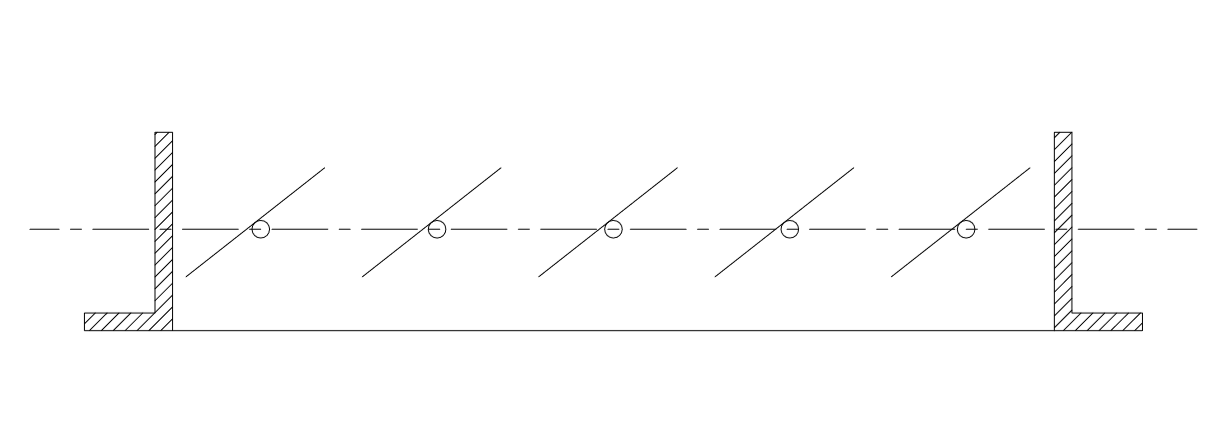
\includegraphics[width=\textwidth]{figure/envctrl.png}
  \caption{散热系统平面图}
  \label{chp:envctrl:end}
\end{figure}
